\scanpage{32}
\margin{31}

Par ces identifications, on trouve une surface topologique \inserted{(\unsure{compacte sans bords})}, dans laquelle la réalisation topologique de $|\Gamma|$ de $\Gamma$ est canoniquement plongée. Les faces orientées de cette surface se réalisent comme les orbites sous l'opération $\rho_f$ sur l'ens \deleted{$\unsure{\vec A}$} $\operatorname{Rep}$ des couples $(\vec a,\omega)$, où $\vec a\in\vec A$, $\omega\in\underline\omega_s\overset{\mathrm{def}}=\underline\omega(\vec A_s)$, opération définie par
\[
\deleted{\rho_f(\vec a,\unsure{\omega})=}
\qquad\text{où }\boxed{\omega_t=\varphi_{\vec a}\omega_s\in\underline\omega(\unsure{A_s|A_t})}
\]
\[
\left\{\begin{aligned}
\rho_f(\vec a,\omega_s)&=(\vec b,\deleted{\unsure{\varphi_{\vec a}\omega_s}}\inserted{\omega_t})\\
\vec b&=\rho_{\omega_t}^{-1}(\deleted{\unsure{\sigma}}-\vec a)
\end{aligned}\right.
\qquad\begin{gathered}\text{et où }b\in\vec A_t\\(t=\operatorname{ex}(\vec a))\\\text{est donné par}\end{gathered}
\]
où $\rho_{\omega_t}$ est la permutation circulaire sur $\vec A_t$ définie par l'orientation $\omega_t$. C'est aussi l'opération de rotation autour des sommets de la carte duale $C^*$, définie par les faces en question.

Si on veut une description combinatoire complète de la carte $C$ définie par $(\Gamma,(\unsure{\pi_s})_{s\in S},(\varphi_{\vec a})_{\vec a\in\vec A})$, il faut expliciter les opérations $\sigma_0,\sigma_1,\sigma_2$ sur $\operatorname{Rep}C$, ens. des repères. On trouve
\margin{str. pol. sur $\vec A_s$}
\[
\left\{\begin{aligned}
\sigma_0(\vec a,\omega_s)&=(-\vec a,-\varphi_{\vec a}\omega_s)\\
\sigma_2(\vec a,\omega_s)&=(\vec a,-\omega_s)\\
\sigma_1(\vec a,\omega_s)&=(\deleted{\unsure{\vec a}}\rho_{\omega_s}(a),-\omega_s)
\end{aligned}\right.
\]
\figure{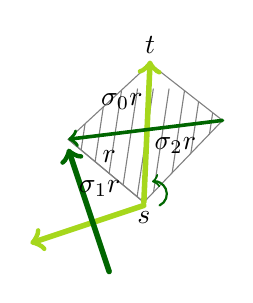
\begin{tikzpicture}[x=.8cm,y=.8cm,line cap=round]
\draw[gray] (0,0)--(-1.2,1)--(.1,2.2)--(1.25,1.3)--cycle;
\draw[gray] (-1.2,1)--(1.25,1.3) (-1.2,1)--(0,0);
\begin{scope}\clip(0,0)--(-1.2,1)--(.1,2.2)--(1.25,1.3)--cycle;\foreach\x in {-1.4,-1.15,...,1.2}{\draw[gray](\x,-.2)--({\x+.3},1.8);}\end{scope}
\draw[yellow!65!green,line width=2pt,->] (0,0)--(.1,2.25);\draw[yellow!65!green,line width=2pt,->] (0,-.05)--(-1.8,-.65);
\draw[green!40!black,line width=2pt,->] (-.55,-1.1)--(-1.2,.85);\draw[green!40!black,line width=1.3pt,->](1.25,1.3)--(-1.2,1);
\draw[green!40!black,thick,->](.25,-.05)arc(-65:100:.2);
\node[below]at(0,0){$s$};\node[above]at(.1,2.2){$t$};\node at(-.55,.72){$r$};\node at(-.35,1.6){$\sigma_0r$};\node at(.5,.9){$\sigma_2r$};\node at(-.7,.22){$\unsure{\sigma_1r}$};
\end{tikzpicture}}

Soit encore, en termes de repères $r$ des $\vec A_s$, en interprétant
\[
\operatorname{Rep}(C)\simeq\coprod_{s\in S}\underbrace{\operatorname{Rep}(\vec A_s)}_{\text{ens des drapeaux}}
\]
\margin{\deleted{\unsure{par le côté}} $\vec a$.}
\[
\left\{\begin{aligned}
\sigma_0(r)&=\deleted{\unsure{(\vec a,\omega)\text{ repère de l'arête}}}\ r',\quad\text{défini par }\left\{\begin{aligned}\unsure{ar_{r'}|a_{r'}}&=-\vec a\\\omega_{r'}&=-\varphi_{\vec a}\omega_r)\end{aligned}\right.\\
\sigma_1(r)&=\widetilde\sigma_0(r)\\
\sigma_2(r)&=\widetilde\sigma_1(r)
\end{aligned}\right.
\]
où $\widetilde\sigma_0^s,\widetilde\sigma_1^s$ sont les opérations sur $\operatorname{Rep}(\vec A_s)$ habituelles, $\widetilde\sigma_i^s$ changeant le composant \inserted{du drapeau} de dimension $i$, pas l'autre.

En termes de ces opérations, on trouve
\[
\left\{\begin{aligned}
\rho_{\mathrm{som}}&=\sigma_2\sigma_{\unsure{1|4}}\deleted{\unsure{\xi}}=\widetilde\sigma_0^s\widetilde\sigma_1^s=\widetilde\rho^s\\
\rho_{\mathrm{face}}&=\sigma_1\sigma_0
\end{aligned}\right.
\]
\inserted{sur $\operatorname{Rep}_s=\operatorname{Rep}(\vec A_s)$}
\margin{opération de rotation \unsure{sur l'ens} des rep. d'un polygone comb.)}
Donc
\[
\rho_{\mathrm{som}}\rho_f=\sigma_2\sigma_0\overset{\mathrm{def}}=\sigma
\qquad\sigma(\vec a,\omega_s)=(-\vec a,\varphi_{\vec a}(\omega_s)).
\]
